\chapter{MOVING TOWARD A 2D ANALYSIS}
\label{app:2D}

One signature of the GMSB models of interest in this analysis
is the presence of two or more high energy jets in the final state.
Using the hadronic activity as a handle to discriminate between signal and background
would be a fruitful way to improve the sensitivity of the analysis. 
In this appendix, I will present a few of the 2D analysis methods
that were explored in the 2016 data set, highlighting the challenges 
that we faced. 

\section{Bin in number of jets}
The simplest method would be to simply bin in jet multiplicity.
This was done in the 8 TeV analysis, but it was dropped in the 
2015 analysis because of the limited size of the data set (2.3 \fbinv).
It was explored in the 2016 analysis, but we decided not 
to pursue it when we made the switch from $ee$ to $ff$ for our 
primary QCD control sample. We are 
already limited enough in $ff$ statistics that binning further 
in the number of jets is not feasible. 

Additionally, there are issues one must address when using 
a discrete variable such as the number of jets. Defining the 
jet ID in such a way that real photons are delineated from 
$e/\gamma$ jet constituents is essential. We also found
that cutting on the number of jets biased the \diempt distribution
in unexpected ways (Figure~\ref{fig:weirdDiempt}).

\begin{figure*}[h]
\begin{center}
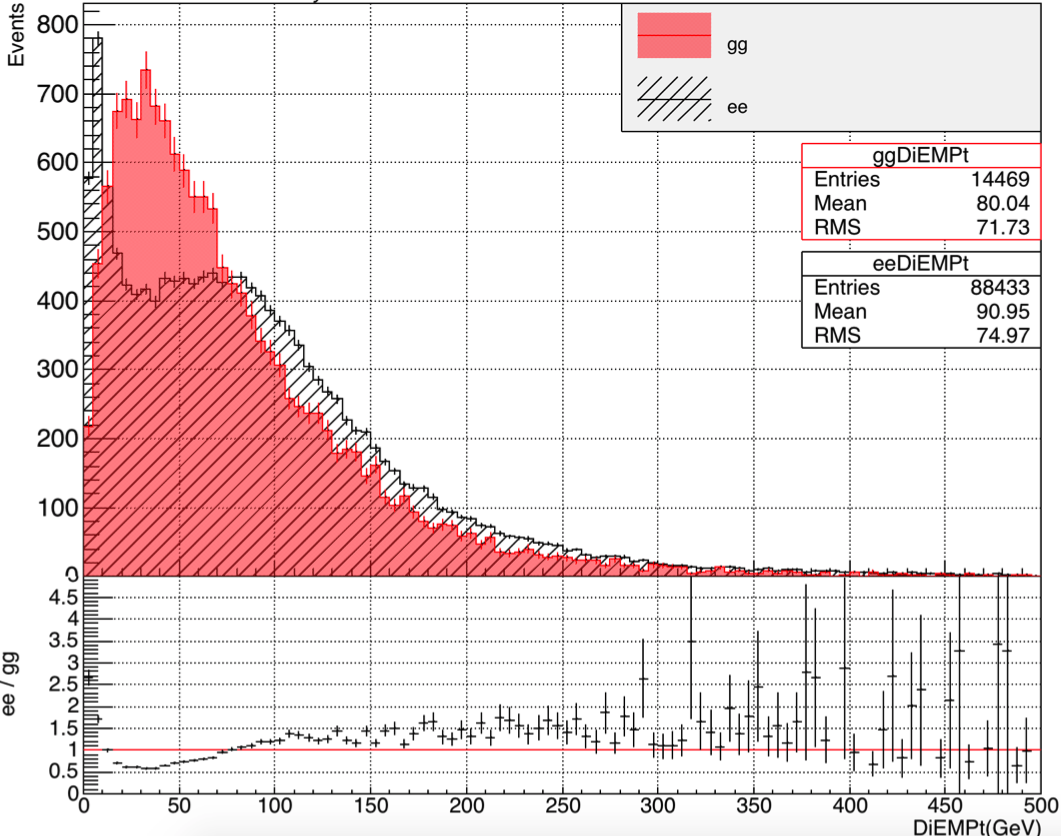
\includegraphics[width=0.9\textwidth]{Figures/Appendix/weirdDiempt.png}
\end{center}
\caption{The \diempt distributions for $\gamma\gamma$ (red) and $ee$ (black)
events with $\geq$ 2 jets. The data corresponds to the first 12.9 \fbinv collected 
with the CMS detector in 2016. The double peak structure only appears if one 
applies a cut on the number of jets. }
\label{fig:weirdDiempt}
\end{figure*}

\section{ABCD method}
The method that we spent the most time exploring is referred to as the ``ABCD" method.
Two discriminating variables are used. The 2D plane is divided into four regions,
as shown in Figure~\ref{fig:ABCD}, where Region $D$ is the signal region and 
Regions $A$--$C$ are control regions with minimal signal contamination.
If the two variables are uncorrelated, then we have the relation
\begin{equation}
\frac{D}{C} = \frac{B}{A}
\end{equation}
which can be rearranged to give a prediction for $D$ in terms of the yields 
in the three control regions:
\begin{equation}
D_{exp}= \frac{BC}{A}
\end{equation}

\begin{figure*}[h]
\begin{center}
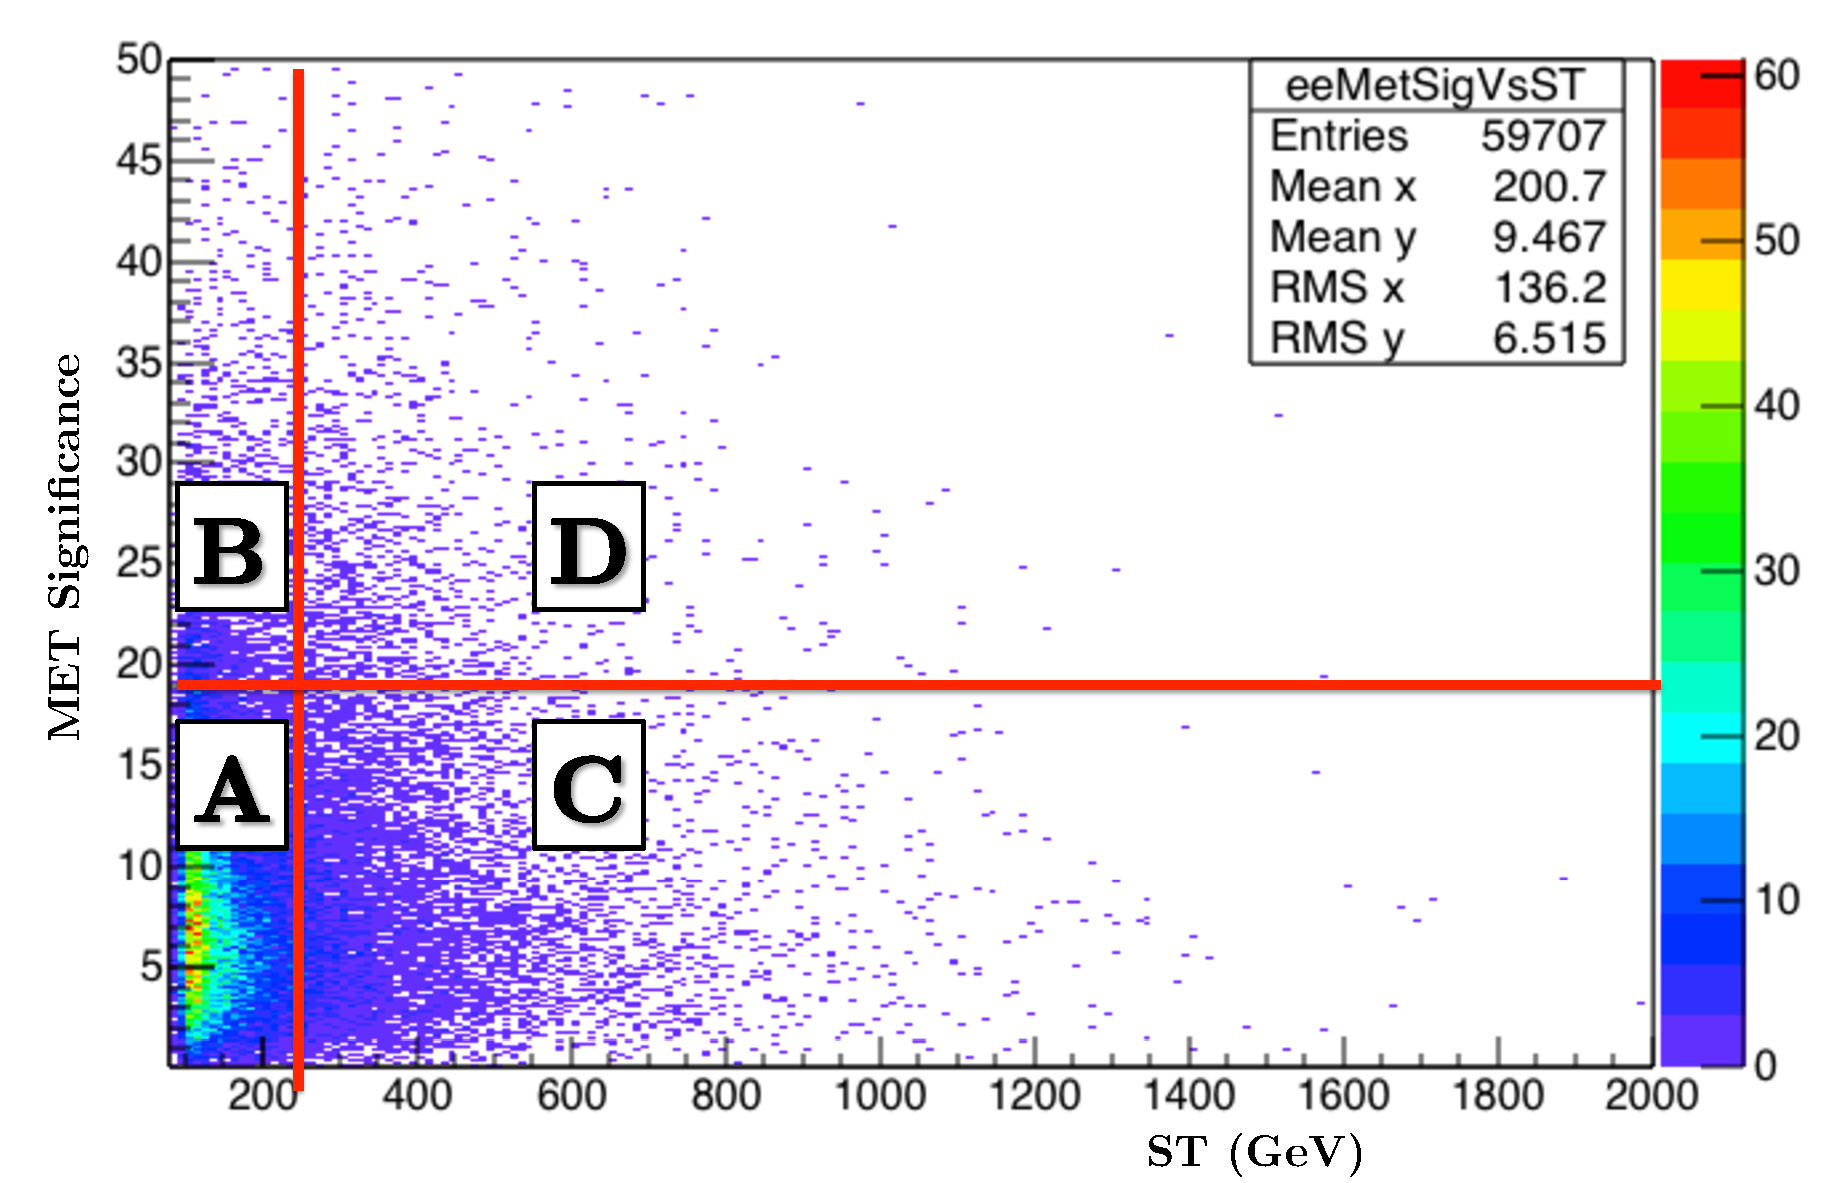
\includegraphics[width=0.9\textwidth]{Figures/Appendix/ABCD_demo.pdf}
\end{center}
\caption{Example of the ABCD analysis method using $ee$ events in data. The two discriminating variables in this plot
are the scalar sum of all visible energy in the event $S_T$, and \ETmiss significance, defined as \ETmiss/$\sqrt{S_T}$. If the two 
variables are uncorrelated, then $D_{exp}= \frac{BC}{A}$.}
\label{fig:ABCD}
\end{figure*}

The problem that we faced was finding two variables that were sufficiently uncorrelated. 
A wide variety of variables were explored:
\begin{itemize}
\item Missing transverse energy \ETmiss
\item $S_T$: scalar sum of the transverse momentum from all photons, leptons, and jets in the event. The sum sometimes includes \ETmiss as well.
\item $H_T$: scalar sum of the transverse momentum from all jets in the event. 
\item \ETmiss significance: Defined as \ETmiss/$\sqrt{S_T}$. This variable quantifies the likelihood that the \ETmiss in an event is real missing energy rather than the result of hadronic mismeasurement. 
\item Missing $H_T$: the magnitude of the vector sum of all photons, leptons, and jets passing our ID criteria.
\item MT2: sometimes referred to as the ``stransverse mass". It is calculated as a function of the two electromagnetic objects and the \ETmiss, and it has a cut-off at the mass of the parents of the invisible particles.
\end{itemize}

To quantify the correlation between two variables $a$ and $b$, I looked at how the ratio 
$N_{a > \alpha}/N_{a < \alpha}$ changes as a function of $b$, where $\alpha$ is the boundary between
regions $AC$ and regions $BD$. The ABCD method relies on the assumption
that this ratio is a constant.
Similarly, one can consider $N_{b > \beta}/N_{b < \beta}$ as a function 
of $a$ for the boundary $\beta$ between $AB$ and $CD$. Figure~\ref{fig:kappa} shows these ratios 
for $S_T$ and \ETmiss significance. Not only are the ratios not constant,
but they exhibit a noticeable change in behavior at $S_T$ = 400 GeV and \ETmiss 
significance = 15. This makes it very difficult to extrapolate the behavior from the control
region to the signal region. Other pairs of variables followed similar trends. 

\begin{figure*}[h]
\begin{center}
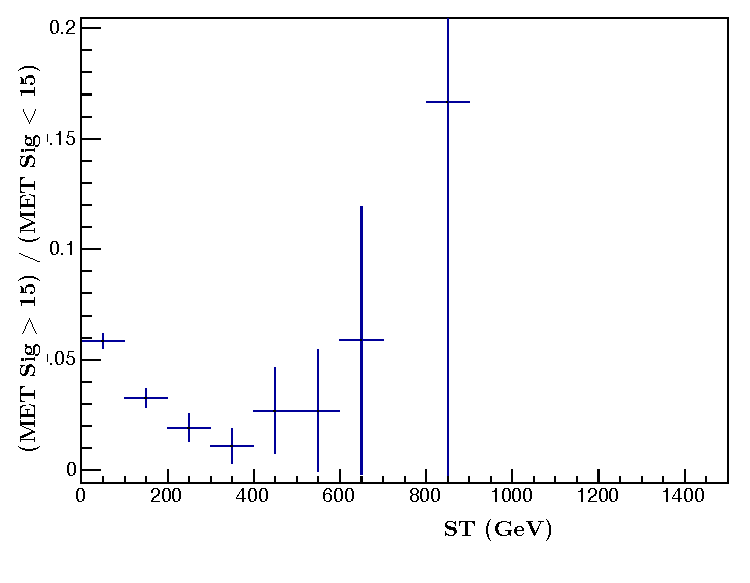
\includegraphics[width=0.49\textwidth]{Figures/Appendix/kappa1.pdf}
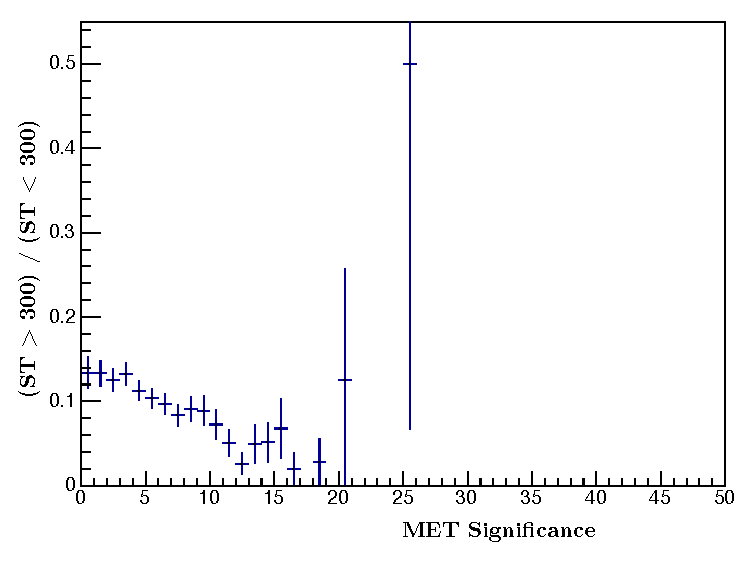
\includegraphics[width=0.49\textwidth]{Figures/Appendix/kappa2.pdf}
\end{center}
\caption{Exploring the correlation between $S_T$ and \ETmiss significance using
the ratio method. If the variables are uncorrelated, the ratios should be constant. These
ratios are for the $ee$ control sample in data.}
\label{fig:kappa}
\end{figure*}

In the end, we decided that it was more important to publish the results and keep to 
a schedule that would allow us to be part of the GMSB combination effort. Efforts at a 
multivariate analysis were tabled until there is time to properly explore it.


%\section{Other ideas}